\section{Jupyter}\label{sec:jupyter}

\subsection{Introduction}

Project Jupyter~\cite{jupyter-project:on,jupyter-doc:on,jupyter-git:on} aims to support
interactive data science and scientific computing across all programming languages. The
notebook~\cite{jupyter-notebook:on} extends the console-based approach to interactive
computing in a qualitatively new direction, providing a web-based application suitable for
capturing the whole computation process: developing, documenting, and executing code, as
well as communicating the results. The Jupyter notebook combines two components:
\begin{enumerate}
\item A web application: a browser-based tool for interactive authoring of documents which
  combine explanatory text, mathematics, computations and their rich media output.
\item Notebook documents: a representation of all content visible in the web application,
  including inputs and outputs of the computations, explanatory text, mathematics, images,
  and rich media representations of objects.
\end{enumerate}
\cite{juplit:on} gives an overview over the best practices for writing (and using)
Jupyter notebooks.

\subsection{What is there?}\label{sec:intro}

\subsubsection{Introduction}
Jupyter is a web application that allows the user to create and share documents that
contain live code, equations, visualizations and explanatory text.

This notebook has among its applications data cleaning and transformation, numerical
simulation, statistical modelling and machine learning. It extends the console-based
approach to interactive computing in a qualitatively new direction, providing a web-based
application suitable for capturing the whole computation process: developing, documenting,
and executing code, as well as communicating the results.

The code that is suitable for this notebook can be written in more than 40 programming
languages, including the most popular ones used in Data Science, such as Python, R, Julia
and Scala.

\subsubsection{History}

Project Jupyter was born out of the IPython Project~\cite{ipython:on,ipython-wikipedia:on}
in 2014 as it evolved to support interactive data science and scientific computing across
all programming languages.  IPython continues to exist as a Python shell and a kernel for
Jupyter, while the notebook and other language-agnostic parts of IPython moved under the
Jupyter name.

IPython was a command shell for interactive computing in multiple programming languages,
originally developed only for Python. It offered introspection, rich media, shell syntax,
tab completion, and history. This interactive computing system provided the following
features:

\begin{itemize}
\item Interactive shells (terminal and Qt-based).
\item A browser-based notebook with support for code, text, mathematical expressions,
  inline plots and other media.
\item Support for interactive data visualization and use of GUI toolkits.
\item Flexible, embeddable interpreters to load into one's own projects.
\item Tools for parallel computing.
\end{itemize}

Jupyter evolved from this and was divided into three major components:
 
\begin{enumerate}
\item A browser-based tool for interactive authoring of documents which combine
  explanatory text, mathematics, computations and their rich media output. This
  application included and extended the features of IPython, leading to new ones:
  \begin{itemize}
  \item In-browser editing for code, with automatic syntax highlighting, indentation, and
    tab completion/introspection.
  \item The ability to execute code from the browser, with the results of computations
    attached to the code which generated them.
  \item Displaying the result of computation using rich media representations, such as
    HTML, LaTeX, PNG, SVG, etc. For example, publication-quality figures rendered by the
    matplotlib library, can be included inline.
  \item In-browser editing for rich text using the Markdown markup language, which can
    provide commentary for the code, is not limited to plain text.
  \item The ability to easily include mathematical notation within markdown cells using
    LaTeX, and rendered natively by MathJax.
  \end{itemize}
	
  %% Notebook documents
\item Notebook documents

  A representation of all content visible in the web application, including inputs and
  outputs of the computations, explanatory text, mathematics, images, and rich media
  representations of objects.


  Notebook documents contain the inputs and outputs of an interactive session as well as
  narrative text that accompanies the code but is not meant for execution. Rich output
  generated by running code, including HTML, images, video, and plots, is embedded in the
  notebook, which makes it a complete and self-contained record of a computation.



  Notebooks consist of a linear sequence of cells. There are three basic cell types:
  \begin{itemize}
  \item Code cells: Input and output of live code that is run in the kernel
  \item Markdown cells: Narrative text with embedded LaTeX equations
  \item Raw cells: Unformatted text that is included, without modification, when notebooks
    are converted to different formats such as LaTeX via nbconvert.
  \end{itemize}

  Notebooks can be exported to different static formats including HTML, reStructeredText,
  LaTeX, PDF, and slide shows. Furthermore, any notebook document, available from a public
  URL qor GitHub, can be shared via ``\textit{nbviewer}''. This service loads the notebook
  document from the URL and renders it as a static web page. The resulting web page may
  thus be shared with others without their needing to install the Jupyter Notebook.

  %% Kernels
\item Kernels:
 
  Through Jupyter's kernel and messaging architecture, the Notebook allows code to be run
  in a range of different programming languages. For each notebook document that a user
  opens, the web application starts a kernel that runs the code for that notebook. Each
  kernel is capable of running code in a single programming language and there are kernels
  available for languages including the following:

\begin{compactitem}
  \item Python: \url{https://github.com/ipython/ipython}
  \item Julia: \url{https://github.com/JuliaLang/IJulia.jl}
  \item R: \url{https://github.com/takluyver/IRkernel}
  \item Ruby: \url{https://github.com/minrk/iruby}
  \item Haskell: \url{https://github.com/gibiansky/IHaskell}
  \item Scala: \url{https://github.com/Bridgewater/scala-notebook}
  \item Node.js: \url{https://gist.github.com/Carreau/4279371}
  \item Go: \url{https://github.com/takluyver/igo}
  \end{compactitem}

  The default kernel runs Python code.  The notebook provides a simple way for users to
  pick which of these kernels is used for a given notebook.

  Each of these kernels communicate with the notebook web application and web browser
  using a JSON over ZeroMQ/WebSockets message protocol.
\end{enumerate}

\subsubsection{Communication Design}

This subsection explains the basic communications design and messaging specification for
how the various Jupyter objects interact over a network transport.  The current
implementation uses the ZeroMQ library for messaging within and between hosts.


\begin{figure}[ht]
  \centering
  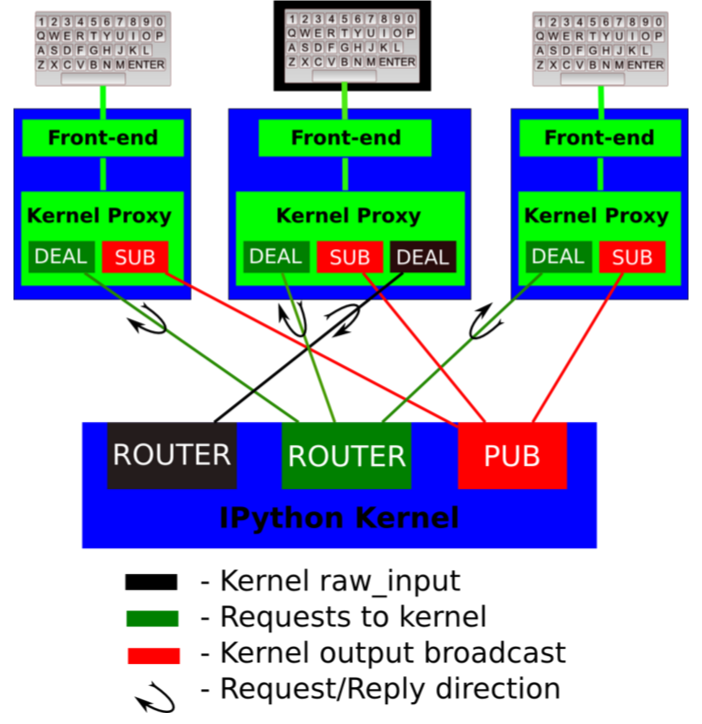
\includegraphics[width=.7\textwidth]{KernelCommunication}
  \caption{The basic design explained}\label{fig:jupyterkernel}
\end{figure} 

A single kernel can be simultaneously connected to one or more frontends. The kernel has
three sockets that serve the following functions:
\begin{enumerate}
\item Shell: This single ROUTER socket allows multiple incoming connections from
  frontends, and this is the socket where requests for code execution, object information,
  prompts, etc.  are made to the kernel by any frontend. The communication on this socket
  is a sequence of request/reply actions from each frontend and the kernel.
\item IOPub: This socket is the "broadcast channel" where the kernel publishes all side
  effects (stdout, stderr etc.) as well as the requests coming from any client over the
  shell socket and its own requests on the stdin socket. There are a number of actions in
  Python which generate side effects: \textit{print()} writes to \textbf{sys.stdout},
  errors generate tracebacks etc. Additionally, in a multi-client scenario, all desire from frontends to be able to know what each other has sent to the kernel (this can be useful
  in collaborative scenarios, for example). This socket allows both side effects and the
  information about communications taking place with one client over the shell channel to
  be made available to all clients in a uniform manner.
\item stdin: This router socket is connected to all frontends, and it allows the kernel to
  request input from the active frontend when \textit{raw-input()} is called. The frontend
  that executed the code has a DEALER socket that acts as a \textit{"virtual keyboard"} for the
  kernel while this communication is happening (illustrated in figure 1 by the black
  outline around the central keyboard). In practice, frontends may display such kernel
  requests using a special input widget or otherwise indicating that the user is to type
  input for the kernel instead of normal commands in the frontend.

  All messages are tagged with enough information for clients to know
  which messages come from their own interaction with the kernel and which ones are from
  other clients, so they can display each type appropriately.
\item Control: This channel is identical to Shell, but operates on a separate socket, to
  allow important messages to avoid queueing behind execution requests (i.e. shutdown or
  abort).
\end{enumerate} 

Messages are dicts of dicts with string keys and values that are reasonably representable
in JSON. The current implementation uses JSON explicitly as its message format, but this
should not be considered a permanent feature. As the JSON has non-trivial performance
issues due to excessive copying, it is plausible that in the future it could move to a
pure pickle-based raw message format. However, it should be possible to easily convert
from the raw objects to JSON, since there may be non-python clients (i.e. a web
frontend). As long as it's easy to make a JSON version of the objects that is a faithful
representation of all the data, a valid communication can be established with such
clients.

\subsection{User Interface}

\subsubsection{Notebook Dashboard}
 
When the jupyter notebook is launched the first page encountered is the Notebook Dashboard. 

\begin{figure}[ht]\centering
  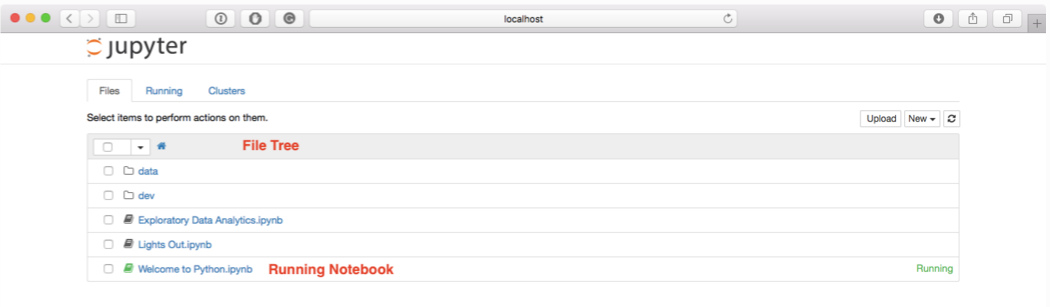
\includegraphics[width=\textwidth]{Dashboard}
  \caption{Jupyter Dashboard}\label{fig:dashboard}
\end{figure} 

\subsubsection{Notebook Editor}
 
Once the user selected a Notebook to edit, the Notebook will open in the Notebook Editor. 

\begin{figure}[ht]\centering
  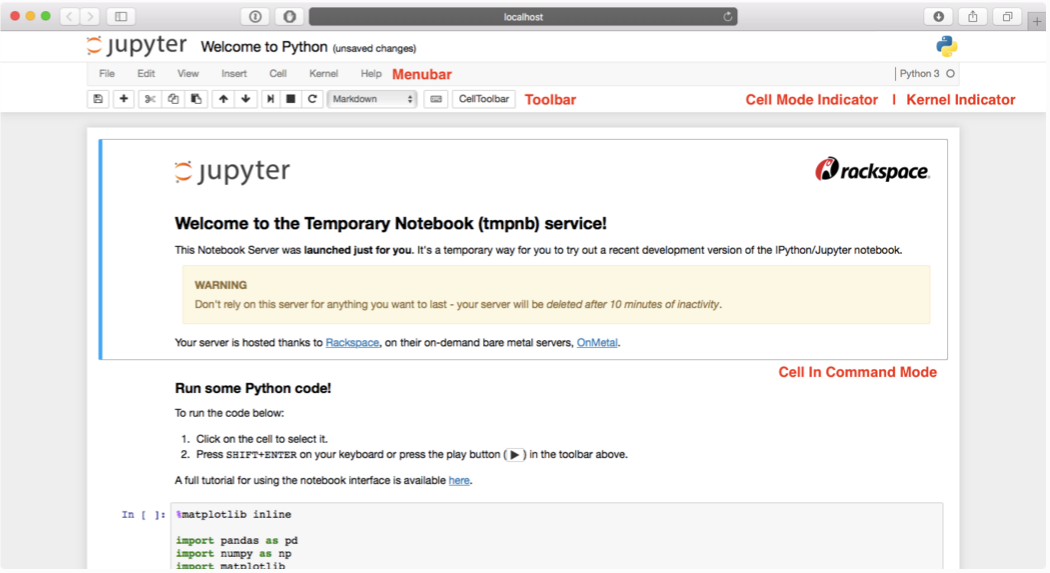
\includegraphics[width=\textwidth]{Editor}
  \caption{Jupyter Editor}\label{fig:editor}
\end{figure} 

\subsubsection{Interactive User Interface Tour of the Notebook}
If the user would like to learn more about the specific elements within the Notebook Editor,
it is possible to take the User Interface Tour by selecting Help in the Menu Bar then selecting User Interface Tour.

\subsubsection{Edit Mode and Notebook Editor}
When a cell is in edit mode, the Cell Mode Indicator will change to reflect the cell’s
state. This state is indicated by a small pencil icon on the top right of the
interface. When the cell is in command mode, there is no icon in that location.

\begin{figure}[ht]\centering
  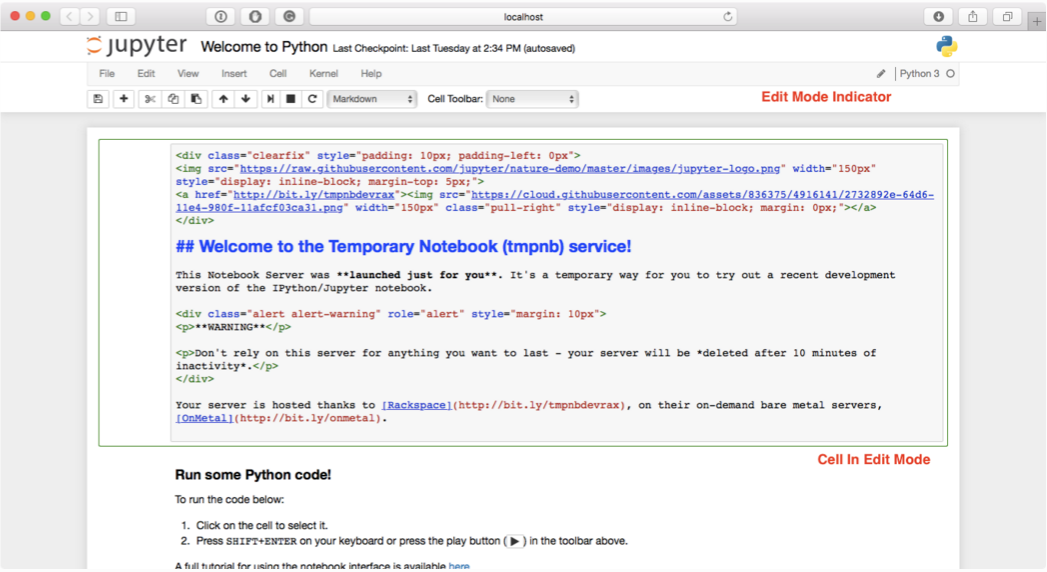
\includegraphics[width=\textwidth]{EditMode}
  \caption{Jupyter Edit Mode}\label{fig:edit-mode}
\end{figure} 

\subsubsection{File Editor }
Now let’s say that the user has chosen to open a Markdown file instead of a Notebook file whilst
in the Notebook Dashboard. If so, the file will be opened in the File Editor.

\subsection{Future Plans for Jupyter}

\subsubsection{Embracing web standards}
By being a pure web application using HTML, Javascript, and CSS, the Notebook can get all
the web technology improvement for free. Thus, as browser support for different media
extend, the notebook web app should be able to be compatible without modification.

This is also true with performance of the User Interface as the speed of Javascript VM increases. 

The other advantage of using only web technology is that the code of the interface is
fully accessible to the end user and is modifiable live. The project strives to keep its
code as accessible and reusable as possible. This should allow the developers to develop
with minimum effort small extensions that customize the behaviour of the web interface.

\subsubsection{Tampering with the Notebook application}

The first tool that is available to the user and that which should be aware of are the
browser ``developers tool''. The exact naming can change across browser and might require
the installation of extensions. But basically they can allow inspection/modifications to
the DOM, and interact with the JavaScript code that runs the frontend.

\subsubsection{Extending the Notebook}
Certain subsystems of the notebook server are designed to be extended or overridden by
users. These documents explain these systems, and show how to override the notebook's
defaults with someone's own custom behaviour.

\subsubsection{Contents API}
This section describes the interface implemented by ContentsManager subclasses. We refer
to this interface as the Contents API.

The Jupyter Notebook web application provides a graphical interface for creating, opening,
renaming, and deleting files in a virtual filesystem.

The ContentsManager class defines an abstract API for translating these interactions into
operations on a particular storage medium. The default implementation,
FileContentsManager, uses the local filesystem of the server for storage and
straightforwardly serializes notebooks into JSON. Users can override these behaviors by
supplying custom subclasses of ContentsManager.

%%% Local Variables:
%%% mode: latex
%%% TeX-master: "report"
%%% End:
